%!TEX root = IntensionalSemantics.tex
\chapter{Propositional Attitudes}\label{cha:propositional_attitudes} % (fold)

\chapterprecishere{We start with the basic possible worlds semantics for
  propositional attitude ascriptions. We talk briefly about the formal
  properties of accessibility relations.}

\minitoc
\excnt=1
\section{Hintikka's Idea} \label{sec:hintikkas-idea}

Expressions %
\sidepar{According to \citet{hintikka:1969:attitudes}, the term
  \term{propositional attitude} goes back to \citet{russell:1940:inquiry}.}%
like \expression{believe}, \expression{know}, \expression{doubt},
\expression{expect}, \expression{regret}, and so on are usually said to describe
\term{propositional attitudes}, expressing relations between individuals (the
attitude holder) and propositions (intensions of sentences).

The simple idea is that \expression{George believes that Henry is a spy} claims
that George believes of the proposition that Henry is a spy that it is true. %
\sidepar{Of course, the possible worlds semantics for propositional attitudes
  was in place long before the extension to fiction contexts was proposed. Our
  discussion here has inverted the historical sequence for pedagogical
  purposes.}%
Note that for the attitude ascription to be true it does not have to hold that
Henry is actually a spy. But where \dash in which world(s) \dash does Henry have
to be a spy for it be true that George believes that Henry is a spy? We might
want to be inspired by the colloquial phrase ``in the world according to
George'' and say that \expression{George believes that Henry is a spy} is true
iff in the world according to George's beliefs, Henry is a spy. We immediately
recall from Chapter 1 that we need to fix this idea up by making space for
multiple worlds compatible with George's beliefs and by tying the
truth-conditions to contingent facts about the evaluation world. That is, what
George believes is different in different possible worlds.

\clearpage The following lexical entry thus offers itself:

\ex $\sv{\mbox{believe}}^{w,g} =\\
\null\hfill\lambda p_{\angles{s,t}}.\ \lambda x. \ \forall w' \mbox{ compatible
  with } x's \mbox{ beliefs in } w\!: p(w') = 1.$ \xe

What %
\sidepar{It is important to realize the modesty of this semantics: we are not
  trying to figure out what belief systems are and particularly not what their
  internal workings are. That is the job of psychologists (and philosophers
  of mind, perhaps). For our semantics, we treat the belief system as a black
  box that determines for each possible world whether it considers it possible
  that it is the world it is located in.}%
is going on in this semantics? We conceive of George's beliefs as a state of his
mind about whose internal structure we will remain agnostic, a matter left to
other cognitive scientists. What we require of it is that it embody opinions
about what the world he is located in looks like. In other words, if his beliefs
are confronted with a particular possible world $w'$, they will determine
whether that world may or may not be the world as they think it is. What we are
asking of George's mental state is whether any state of affairs, any event,
anything in $w'$ is in contradiction with anything that George believes. If not,
then $w'$ is compatible with George's beliefs. For all George believes, $w'$ may
well be the world where he lives. Many worlds will pass this criterion, just
consider as one factor that George is unlikely to have any precise opinions
about the number of leaves on the tree in front of my house. George's belief
system determines a set of worlds compatible with his beliefs: those worlds that
are viable candidates for being the actual world, as far as his belief system is
concerned.

Now, George believes a proposition iff that proposition is true in all of the
worlds compatible with his beliefs. If there is just one world compatible with
his beliefs where the proposition is not true, that means that he considers it
possible that the proposition is not true. In such a case, we can't say that he
believes the proposition. Here is the same story in the words of
\citet{hintikka:1969:attitudes}, the source for this semantics for propositional
attitudes:

% The picture of Hintikka here is from his Helsinki homepage: http://www.helsinki.fi/filosofia/filo/henk/hintikka.htm.

\begin{quotation}
	
  My %
  \sidepar{\centering
\includegraphics[height=1in]{hintikka1.JPG}\\
    {\tiny \href{http://www.helsinki.fi/filosofia/filo/henk/hintikka.htm}{Jaakko
        Hintikka}}}%
  basic assumption (slightly simplified) is that an attribution of any
  propositional attitude to the person in question involves a division of all
  the possible worlds (\dots) into two classes: into those possible worlds which
  are in accordance with the attitude in question and into those which are
  incompatible with it. The meaning of the division in the case of such
  attitudes as knowledge, belief, memory, perception, hope, wish, striving,
  desire, etc. is clear enough. For instance, if what we are speaking of are
  (say) $a$'s memories, then these possible worlds are all the possible worlds
  compatible with everything he remembers. [\dots]
	
	How are these informal observations to be incorporated into a more explicit
  semantical theory? According to what I have said, understanding attributions
  of the propositional attitude in question (\dots) means being able to make a
  distinction between two kinds of possible worlds, according to whether they
  are compatible with the relevant attitudes of the person in question. The
  semantical counterpart to this is of course a function which to a given
  individual person assigns a set of possible worlds.
	
	However, a minor complication is in order here. Of course, the person in
  question may himself have different attitudes in the different worlds we are
  considering. Hence this function in effect becomes a relation which to a given
  individual and to a given possible world $\mu$ associates a number of possible
  worlds which we shall call the \term{alternatives} to $\mu$. The relation will
  be called the alternativeness relation. (For different propositional
  attitudes, we have to consider different alternativeness relations.)
\end{quotation}

\begin{exercise}
	
	Let's adopt Hintikka's idea that we can use a function that maps $x$ and $w$
  into the set of worlds $w'$ compatible with what $x$ believes in $w$. Call
  this function $\mathcal{B}$. That is,
	
	\ex $\mathcal{B} = \lambda x.\ \lambda w.\ \{w'\co w' \mbox{ is compatible
    with what } x \mbox{ believes in } w\}.$ \xe
%	
	Using this notation, our lexical entry for \expression{believe} would look as
  follows:
	
	\ex $\sv{\mbox{believe}}^{w,g} = \lambda p_{\angles{s,t}}.\ \lambda x.\
  \mathcal{B}(x)(w) \subseteq p.$ \xe
%	
	We are here indulging in the usual sloppiness in treating $p$ both as a
  function from worlds to truth-values and as the set characterized by that
  function.
	
	Here now are two ``alternatives'' for the semantics of \expression{believe}:
	
	\ex \extitle{Attempt 1 (very wrong)}\\[3pt]
	$\sv{\mbox{believe}}^{w,g} = \lambda p \in D_{\angles{s,t}}. \big[ \lambda x
  \in D.\ p = \mathcal{B}(x)(w) \big]$. \xe
	
	\ex \extitle{Attempt 2 (also very wrong)}\\[3pt]
	$\sv{\mbox{believe}}^{w,g} = \lambda p \in D_{\angles{s,t}}. \big[ \lambda x
  \in D.\ p \cap \mathcal{B}(x)(w) \neq \emptyset \big]$. \xe
%	
	Explain why these do not adequately capture the meaning of
  \expression{believe}. \eex
\end{exercise}
%
\begin{exercise}
  Follow-up: The semantics in (\lastx) would have made \emph{believe} into an
  existential quantifier of sorts: it would say that \emph{some} of the worlds
  compatible with what the subject believes are such-and-such. You have argued
  (successfully, of course) that such an analysis is wrong for \emph{believe}.
  But \emph{are} there attitude predicates with such an ``existential'' meaning?
  Discuss some candidates. If you can't find any candidates that survive
  scrutiny, can you speculate why there might be no existential attitude
  predicates? [Warning: this is underexplored territory!] \eex
\end{exercise}
%
\clearpage We can also think of belief states as being represented by a function
$\mathcal{BS}$\sidepar{$\mathcal{BS}$ is meant to stand for
  `\underline{\bfseries b}elief \underline{\bfseries s}tate', not for what you
  might have thought!}, which maps an individual and a world into a set of
propositions: those that the individual believes. From there, we could calculate
the set of worlds compatible with an individual $x$'s beliefs in world $w$ by
retrieving the set of those possible worlds in which all of the propositions in
$\mathcal{BS}(x)(w)$ are true: $\{w': \forall p \in \mathcal{BS}(x)(w): p(w') =
1\}$, which in set talk is simply the big intersection of all the propositions
in the set: $\cap \mathcal{BS}(x)(w)$. Our lexical entry then would be:

\ex $\sv{\mbox{believe}}^{w,g} = \lambda p_{\angles{s,t}}.\ \lambda x. \cap
\mathcal{BS}(x)(w) \subseteq p.$ \xe

\begin{exercise}
	
	Imagine that our individual $x$ forms a new opinion. Imagine that we model
  this by adding a new proposition $p$ to the pool of opinions. So,
  $\mathcal{BS}(x)(w)$ now contains one further element. There are now more
  opinions. What happens to the set of worlds compatible with $x$'s beliefs?
  Does it get bigger or smaller? Is the new set a subset or superset of the
  previous set of compatible worlds? \eex
\end{exercise}

\section{Accessibility Relations} \label{sec:access-relat}

Another way of reformulating Hintikka's semantics for propositional attitudes is
via the notion of an \term{accessibility relation}. We talk of a world $w'$
being accessible from $w$. Each attitude can be associated with such an
accessibility relation. For example, we can introduce the relation
$w\mathcal{R}^{\mathcal{B}}_{a}w'$ which holds iff $w'$ is compatible with $a$'s
belief state in $w$. We have then yet another equivalent way of specifying the
lexical entry for \expression{believe}:

\ex $\sv{\mbox{believe}}^{w,g} = \lambda p_{\angles{s,t}}.\ \lambda x. \ \forall
w': w\mathcal{R}^{\mathcal{B}}_{x}w' \rightarrow p(w') = 1.$ \xe

It is profitable to think of different attitudes (belief, knowledge, hope,
regret, memory, \dots) as corresponding to different accessibility relations.
Recall now %
\sidepar{Kirill Shklovsky (in class) asked why we call reflexivity,
  transitivity, and symmetry ``formal'' properties of relations. The idea is
  that certain properties are ``formal'' or ``logical'', while others are more
  substantial. So, the fact that the relation ``have the same birthday as'' is
  symmetric seems a more formal fact about it than the fact that the relation
  holds between my daughter and my brother-in-law. Nevertheless, one of the most
  common ways of characterizing formal/logical notions (permutation-invariance,
  if you're curious) does not in fact make symmetry etc. a formal/logical
  notion. So, while intuitively these do seem to be formal/logical properties,
  we do not know how to substantiate that intuition. See
  \citet{macfarlane:2005:logical-constants} for discussion.}%
that the linguistic study of determiners benefitted quite a bit from an
investigation of the formal properties of the relations between sets of
individuals that determiners express. We can do the same thing here and ask
about the formal properties of the accessibility relation associated with belief
versus the one associated with knowledge, etc. The obvious properties to think
about are reflexivity, transitivity, and symmetry.

\subsection{Reflexivity} \label{sec:reflexivity}

A relation is reflexive iff for any object in the domain of the relation we know
that the relation holds between that object and itself. Which accessibility
relations are reflexive? Take knowledge:

\ex $w\mathcal{R}^{\mathcal{K}}_{x}w'$ iff $w'$ is compatible with what $x$
knows in $w$. \xe

We %
\marginnote{We talk here about knowledge entailing (or even presupposing) truth but
  we do not mean to say that knowledge simply equals true belief. Professors
  Socrates and Gettier and their exegetes have further considerations.}%
are asking whether for any given possible world $w$, we know that
$\mathcal{R}^{\mathcal{K}}_{x}$ holds between $w$ and $w$ itself. It will hold
if $w$ is a world that is compatible with what we know in $w$. And clearly that
must be so. Take our body of knowledge in $w$. The concept of knowledge
crucially contains the concept of truth: what we know must be true. So if in $w$
we know that something is the case then it must be the case in $w$. So, $w$ must
be compatible with all we know in $w$. $\mathcal{R}^{\mathcal{K}}_{x}$ is
reflexive.

Now, if an attitude $X$ corresponds to a reflexive accessibility relation, then
we can conclude from \expression{$a$ $Xs$ that $p$} being true in $w$ that $p$
is true in $w$. %
\sidepar{In modal logic notation: $\square p \rightarrow p $. This pattern is
  sometimes called \textbf{T} or \textbf{M}, as is the corresponding system of
  modal logic.}%
This property of an attitude predicate is often called \term{veridicality}. It
is to be distinguished from \term{factivity}, which is a property of attitudes
which \emph{presuppose} -- rather than (merely) entail -- the truth of their
complement.

If we consider the relation $\mathcal{R}^\mathcal{B}_{x}$ pairing with a world
$w$ those worlds $w'$ which are compatible with what $x$ \emph{believes} in $w$,
we no longer have reflexivity: belief is not a veridical attitude. %
\sidepar{The difference between \emph{believe} and \emph{know} in natural
  discourse is quite delicate, especially when one considers first person uses
  (\emph{I believe the earth is flat} vs. \emph{I know the earth is flat}).}%
It is easy to have false beliefs, which means that the actual world is not in
fact compatible with one's beliefs, which contradicts reflexivity. And many
other attitudes as well do not involve veridicality/reflexivity: what we hope
may not come true, what we remember may not be what actually happened, etc.

In modal logic, the correspondence between formal properties of the
accessibility relation and the validity of inference patterns is well-studied.
What we have just seen is that reflexivity of the accessibility relation
corresponds to the validity of $\square p \rightarrow p$. Other properties
correspond to other characteristic patterns. Let's see this for transitivity and
symmetry.

\subsection{*Transitivity} \label{sec:transitivity}

Transitivity of the accessibility relation corresponds to the inference $\square
p \rightarrow \square \square p$.\sidepar{In the literature on epistemic modal
  logic, the pattern is known as the \term{KK Thesis} or \term{Positive
    Introspection}. In general modal logic, it is the characteristic axiom
  \textbf{4} of the modal logic system \textbf{S4}, which is a system that adds
  \textbf{4} to the previous axiom \textbf{M}/\textbf{T}. Thus, \textbf{S4} is
  the logic of accessibility relations that are both reflexive and transitive.}
The pattern seems not obviously wrong for knowledge: if one knows that $p$,
doesn't one thereby know that one knows that $p$? But before we comment on that,
let's establish the formal correspondence between transitivity and that
inference pattern. This needs to go in both directions.
  
\begin{figure}[htbp]
  \centering
    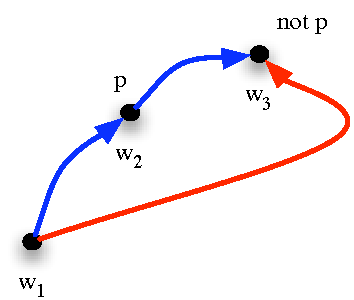
\includegraphics[height=1.5in]{transitivity.pdf}
  \caption{Transitivity}
  \label{fig:transitivity}
\end{figure}

\noindent What does it take for the pattern to be valid? Assume that $\square p$
holds for an arbitrary world $w$, i.e. that $p$ is true in all worlds $w'$
accessible from $w$. Now, the inference is to the fact that $p$ again holds in
any world $w''$ accessible from any of those worlds $w'$ accessible from $w$.
But what would prevent $p$ from being false in some $w''$ accessible from some
$w'$ accessible from $w$? That could only be prevented from happening if we knew
that $w''$ itself is accessible from $w$ as well, because then we would know
from the premiss that $p$ is true in it (since $p$ is true in \emph{all} worlds
accessible from $w$). Ah, but $w''$ (some world accessible from a world $w'$
accessible from $w$) is only guaranteed to be accessible from $w$ if the
accessibility relation is transitive (if $w'$ is accessible from $w$ and $w''$
is accessible from $w'$, then transitivity ensures that $w''$ is accessible from
$w$). This reasoning has shown that validity of the pattern requires
transitivity. The other half of proving the correspondence is to show that
transitivity entails that the pattern is valid.

The proof proceeds by reductio. Assume that the accessibility relation is
transitive. Assume that (i) $\square p$ holds for some world $w$ but that (ii)
$\square \square p$ doesn't hold in $w$. We will show that this situation cannot
obtain. By (i), $p$ is true in all worlds $w'$ accessible from $w$. By (ii),
there is some non-$p$ world $w''$ accessible from some world $w'$ accessible
from $w$. But by transitivity of the accessibility relation, that non-$p$ world
$w''$ must be accessible from $w$. And since \emph{all} worlds accessible from
$w$ are $p$ worlds, $w''$ must be a $p$ world, in contradiction to (ii). So, as
soon as we assume transitivity, there is no way for the inference not to go
through.

Now, do any of the attitudes have the transitivity property? It seems rather
obvious that as soon as you believe something, you thereby believe that you
believe it (and so it seems that belief involves a transitive accessibility
relation). And in fact, as soon as you believe something, you believe that you
\emph{know} it. But one might shy away from saying that knowing something
automatically amounts to knowing that you know it. For example, many are
attracted to the idea that to know something requires that (i) that it is true,
(ii) that you believe it, and (iii) that you are justified in believing it: the
justified true belief analysis of knowledge. So, now couldn't it be that you
know something, and thus (?) that you believe you know it, and thus that you
believe that you are justified in believing it, but that you are not justified
in believing that you are \emph{justified} in believing it? After all, one's
source of knowledge, one's reliable means of acquiring knowledge, might be a
mechanism that one has no insight into. So, while one can implicitly trust
(believe) in its reliability, and while it is in fact reliable, one might not
have any means to have trustworthy beliefs about it. [Further worries about the
KK Thesis are discussed by \citet{williamson:2000:limits}.]

\subsection{*Symmetry}

What would the consequences be if the accessibility relation were symmetric?
Symmetry of the accessibility relation $\mathcal{R}$ corresponds to the validity
of the following principle:
%
\marginnote{In modal logic notation: $p \rightarrow \square\diamondsuit p$, known
  simply as B in modal logic. The system that combines \textbf{T}/\textbf{M}
  with B is often called Brouwer's System (\textbf{B}), after the mathematician
  L.E.J. Brouwer, not because he proposed it but because it was thought that it
  had some connections to his doctrines.}%
\ex Brouwer's Axiom :\\
$\forall p \forall w:\ w\in p \rightarrow \Bigl[\forall w' \bigl[ w\mathcal{R}w'
\rightarrow \exists w'' \left[ w'\mathcal{R}w'' \&\ w''\in p\right]\bigr]\Bigr]$ \xe
%
% Brouwer photo from
% http://www-gap.dcs.st-and.ac.uk/~history/Mathematicians/Brouwer.html
% O. Becker in "Zur Logik der Modalitäten" (Jahrbuch für Philosophie
% und Phänomenologische Forschung, vol. 11 (1930), 497-548, called
% this Brouwer's axiom.) 

\marginpar{\centering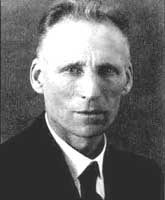
\includegraphics[height=1in]{Brouwer.jpg}\\
  {\tiny \href{http://plato.stanford.edu/entries/brouwer/}{L.E.J. Brouwer}}}%
\begin{figure}[htbp]
  \centering
    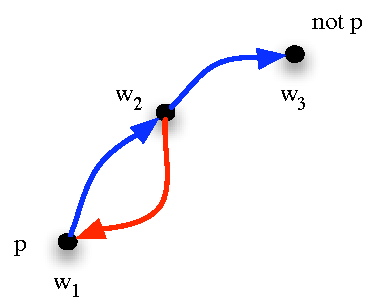
\includegraphics[height=1.5in]{symmetry.pdf}
  \caption{Symmetry}
  \label{fig:symmetry}
\end{figure}
%
Here's the reasoning: Assume that $R$ is in fact symmetric. Pick a world $w$ in
which $p$ is true. Now, could it be that the right hand side of the inference
fails to hold in $w$? Assume that it does fail. Then, there must be some world
$w'$ accessible from $w$ in which $\diamondsuit p$ is false. In other words,
from that world $w'$ there is no accessible world $w''$ in which $p$ is true.
But since $R$ is assumed to be symmetric, one of the worlds accessible from $w'$
is $w$ and in $w$, $p$ is true, which contradicts the assumption that the
inference doesn't go through. So, symmetry ensures the validity of the
inference.

The other way (validity of the inference requires symmetry): the inference says
that from any $p$ world we only have worlds accessible from which there is at
least one accessible $p$ world. But imagine that $p$ is true in $w$ but not true
in any other world. So, the only way for the conclusion of the inference to hold
automatically is to have a guarantee that $w$ (the only $p$ world) is accessible
from any world accessible from it. That is, we need to have symmetry. QED.

To see whether a particular kind of attitude is based on a symmetric
accessibility relation, we can ask whether Brouwer's Axiom is intuitively valid
with respect to this attitude. If it is not valid, this shows that the
accessibility relation can't be symmetric. In the case of a knowledge-based
accessibility relation (epistemic accessibility), one can argue that
\emph{symmetry does not hold}:\footnote{Thanks to Bob Stalnaker (pc to Kai von
  Fintel) for help with the following reasoning.}
\begin{quote}
  
  The symmetry condition would imply that if something happens to be true in the
  actual world, then you know that it is compatible with your knowledge
  (Brouwer's Axiom). This will be violated by any case in which your beliefs are
  consistent, but mistaken. Suppose that while $p$ is in fact true, you feel
  certain that it is false, and so think that you know that it is false. Since
  you think you know this, it is compatible with your knowledge that you know
  it. (Since we are assuming you are consistent, you can't both believe that you
  know it, and know that you do not). So it is compatible with your knowledge
  that you know that \expression{not} $p$. Equivalently\footnote{This and the
    following step rely on the duality of necessity and possibility: $q$ is
    compatible with your knowledge iff you don't know that \expression{not}
    $q$.}: you don't know that you don't know that \expression{not} $p$.
  Equivalently: you don't know that it's compatible with your knowledge that
  $p$. But by Brouwer's Axiom, since $p$ is true, you would have to know that
  it's compatible with your knowledge that $p$. So if Brouwer's Axiom held,
  there would be a contradiction. So Brouwer's Axiom doesn't hold here, which
  shows that epistemic accessibility is not symmetric.
\end{quote}

\noindent Game theorists and theoretical computer scientists who traffic in
logics of knowledge often assume that the accessibility relation for knowledge
is an equivalence relation (reflexive, symmetric, and transitive). But this is
appropriate only if one abstracts away from any error, in effect assuming that
belief and knowledge coincide. One\sidepar{All one really needs to make
  \textbf{NI} valid is to have a \term{Euclidean} accessibility relation: any
  two worlds accessible from the same world are accessible from each other. It
  is a nice little exercise to prove this, if you have become interested in this
  sort of thing. Note that all reflexive and Euclidean accessibility relations
  are transitive and symmetric as well \dash another nice little thing to
  prove.} striking consequence of working with an equivalence relation as the
accessibility relation for knowledge is that one predicts the principle of
\term{Negative Introspection} to hold:

\ex \extitle{Negative Introspection (\textbf{ni})}\\
If one doesn't know that $p$, then one knows that one doesn't know that $p$.
($\neg\square p \rightarrow \square\neg\square p$). \xe

This surely seems rather dubious: imagine that one strongly believes that $p$
but that nevertheless $p$ is false, then one doesn't know that $p$, but one
doesn't seem to believe that one doesn't know that $p$, in fact one believes
that one does know that $p$.

% \section{A Note on Shortcomings} \label{sec:note-shortcomings}
% 
% [ \dots to be written \dots stuff about \term{hyperintensionality} ]

%POSSIBLE EXERCISE: SHOW THAT NEGATION CANNOT BE TREATED AS SHIFTING US TO THE SET OF WORLDS WHERE THINGS ARE THE OPPOSITE OF THE WAY THEY ARE IN THE EVALUATION WORLD. OR IS THAT TOO CRAZY?

\section{Supplemental Readings}

{\setlength{\parindent}{0pt}\setlength{\parskip}{6pt}

  % We will come back to propositional attitudes and especially the
  % scope of noun phrases with respect to them, including the infamous
  % \term{de dicto}-\term{de re} distinction.

A recent survey on attitudes:
\begin{bibentrylist}
	\item \bibentry{swanson-2011-hsk-attitudes}.
\end{bibentrylist}

Further connections between mathematical properties of accessibility relations
and logical properties of various notions of necessity and possibility are
studied extensively in modal logic:
\begin{bibentrylist}
  \item \bibentry{hughes-cresswell:1996:new}. 
  \item \bibentry{garson:2003:logic-modal}, especially section 7 and 8, ``Modal Axioms and Conditions on Frames'', ``Map of the Relationships between Modal Logics''. 
\end{bibentrylist}

A thorough discussion of the possible worlds theory of attitudes, and some of
its potential shortcomings, can be found in Bob Stalnaker's work:
\begin{bibentrylist}
	\item \bibentry{stalnaker:1984:inquiry}. 
	\item \bibentry{stalnaker:1999:contextandcontent}. 
\end{bibentrylist}

A quick and informative surveys about the notion of knowledge:
\begin{bibentrylist}
	\item \bibentry{steup:2008:knowledge}. 
\end{bibentrylist}

Linguistic work on attitudes has often been concerned with various co-occurrence
patterns, particularly which moods (indicative or subjunctive or infinitive)
occur in the complement and whether negative polarity items are licensed in the
complement.

Mood licensing:
\begin{bibentrylist}
	\item \bibentry{portner:1997:mood}. 
\end{bibentrylist}

NPI-Licensing:
\begin{bibentrylist}
	\item \bibentry{kadmon-landman:1993:any}. 
	\item \bibentry{fintel:1999:npi}.
  \item \bibentry{giannakidou:1999:affective}. 
\end{bibentrylist}

There is some interesting work out of Amherst rethinking the way attitude
predicates take their complements:

\begin{bibentrylist}
  \item \bibentry{kratzer:2006:decomposing}.
  \item \bibentry{moulton:2008:wager}. \url{http://people.umass.edu/keir/Wager.pdf}.
  \item \bibentry{moulton:2009:thesis}.
\end{bibentrylist}

Tamina Stephenson in her MIT dissertation and related work explores the way
attitude predicates interact with epistemic modals and taste predicates in their
complements:

\begin{bibentrylist}
  \item \bibentry{stephenson:2007:judge-lp}.
  \item\bibentry{stephenson:2007:thesis}.
\end{bibentrylist}

Jon Gajewski in his MIT dissertation and subsequent work explores the
distribution of the \term{neg-raising} property among attitude predicates and
traces it back to presuppositional components of the meaning of the predicates:

\begin{bibentrylist}
	\item \bibentry{gajewski:2005:thesis}.
	\item \bibentry{gajewski:2007:neg-raising}.
\end{bibentrylist}

Interesting work has also been done on presupposition projection in attitude
contexts:
\begin{bibentrylist}
	\item \bibentry{asher:1987:attitudes}.
	\item \bibentry{heim:1992:attitude}. 
	\item \bibentry{geurts:1998:attitudes}. 
\end{bibentrylist}

}

% chapter propositional_attitudes (end)

